\documentclass[addpoints,12pt]{exam}\usepackage[]{graphicx}\usepackage[]{color}
%% maxwidth is the original width if it is less than linewidth
%% otherwise use linewidth (to make sure the graphics do not exceed the margin)
\makeatletter
\def\maxwidth{ %
  \ifdim\Gin@nat@width>\linewidth
    \linewidth
  \else
    \Gin@nat@width
  \fi
}
\makeatother

\definecolor{fgcolor}{rgb}{0.345, 0.345, 0.345}
\newcommand{\hlnum}[1]{\textcolor[rgb]{0.686,0.059,0.569}{#1}}%
\newcommand{\hlstr}[1]{\textcolor[rgb]{0.192,0.494,0.8}{#1}}%
\newcommand{\hlcom}[1]{\textcolor[rgb]{0.678,0.584,0.686}{\textit{#1}}}%
\newcommand{\hlopt}[1]{\textcolor[rgb]{0,0,0}{#1}}%
\newcommand{\hlstd}[1]{\textcolor[rgb]{0.345,0.345,0.345}{#1}}%
\newcommand{\hlkwa}[1]{\textcolor[rgb]{0.161,0.373,0.58}{\textbf{#1}}}%
\newcommand{\hlkwb}[1]{\textcolor[rgb]{0.69,0.353,0.396}{#1}}%
\newcommand{\hlkwc}[1]{\textcolor[rgb]{0.333,0.667,0.333}{#1}}%
\newcommand{\hlkwd}[1]{\textcolor[rgb]{0.737,0.353,0.396}{\textbf{#1}}}%


\makeatletter
\newenvironment{kframe}{%
 \def\at@end@of@kframe{}%
 \ifinner\ifhmode%
  \def\at@end@of@kframe{\end{minipage}}%
  \begin{minipage}{\columnwidth}%
 \fi\fi%
 \def\FrameCommand##1{\hskip\@totalleftmargin \hskip-\fboxsep
 \colorbox{shadecolor}{##1}\hskip-\fboxsep
     % There is no \\@totalrightmargin, so:
     \hskip-\linewidth \hskip-\@totalleftmargin \hskip\columnwidth}%
 \MakeFramed {\advance\hsize-\width
   \@totalleftmargin\z@ \linewidth\hsize
   \@setminipage}}%
 {\par\unskip\endMakeFramed%
 \at@end@of@kframe}
\makeatother

\definecolor{shadecolor}{rgb}{.97, .97, .97}
\definecolor{messagecolor}{rgb}{0, 0, 0}
\definecolor{warningcolor}{rgb}{1, 0, 1}
\definecolor{errorcolor}{rgb}{1, 0, 0}
\newenvironment{knitrout}{}{} % an empty environment to be redefined in TeX

\usepackage{alltt}
\usepackage{amsmath, amssymb}
\linespread{1.1}
\usepackage{hyperref}
\usepackage{enumerate}
\usepackage{multirow}



%-------------------DON'T CHANGE---------------------%
%The following is needed to prevent a conflict between knitr and the exam class involving the package ``framed.''



%This keeps images from being too big, centers them, and makes sure we use pdf images



%Change the default width of the output to fit within the solution boxes

%-------------------DON'T CHANGE---------------------%


%To include the answers use:
%  pdflatex "\def\showanswers{1} \input{thisfile.tex}"
%\ifdefined\showanswers
  \printanswers
%\else
 % \noprintanswers
%\fi

\title{Extra Credit Problem}
\author{Econ 103}
\date{}
\IfFileExists{upquote.sty}{\usepackage{upquote}}{}
\begin{document}
\maketitle

\section*{Regression with R}
\begin{questions}

\question This question is based on the dataset on child test scores and mother characteristics. You can download the data with the following code:

\begin{knitrout}
\definecolor{shadecolor}{rgb}{0.969, 0.969, 0.969}\color{fgcolor}\begin{kframe}
\begin{alltt}
\hlstd{data.url} \hlkwb{<-} \hlstr{'http://www.ditraglia.com/econ103/child_test_data.csv'}
\hlstd{data} \hlkwb{<-} \hlkwd{read.csv}\hlstd{(data.url)}
\hlkwd{head}\hlstd{(data)}
\end{alltt}
\begin{verbatim}
##   kid.score mom.hs    mom.iq mom.age
## 1        65      1 121.11753      27
## 2        98      1  89.36188      25
## 3        85      1 115.44316      27
## 4        83      1  99.44964      25
## 5       115      1  92.74571      27
## 6        98      0 107.90184      18
\end{verbatim}
\begin{alltt}
\hlkwd{attach}\hlstd{(data)}
\end{alltt}
\end{kframe}
\end{knitrout}
\vspace{0.2in}
The columns contained in this dataset are as follows:
\begin{table}[h]
\centering
	\begin{tabular}{ll}
		Variable Name & Description\\
		\hline
		\texttt{kid.score}& Child's Test Score at Age 3\\
		\texttt{mom.age}&Age of Mother at Birth of Child\\
		\texttt{mom.hs}& Mother Completed High School? (1 = Yes)\\
		\texttt{mom.iq}& Mother's IQ Score
	\end{tabular}
\end{table}
\newpage
	\begin{parts}
		\part Run a regression of \texttt{kid.score} on \texttt{mom.age}. Plot both the data and the fitted regression line, making sure to label the axes  (Check R tutorial 3). \underline{Interpret the results}. 
    \begin{solution}
\begin{knitrout}
\definecolor{shadecolor}{rgb}{0.969, 0.969, 0.969}\color{fgcolor}\begin{kframe}
\begin{alltt}
\hlstd{reg1} \hlkwb{<-} \hlkwd{lm}\hlstd{(kid.score} \hlopt{~} \hlstd{mom.age)}
\hlkwd{summary}\hlstd{(reg1)}
\end{alltt}
\begin{verbatim}
## 
## Call:
## lm(formula = kid.score ~ mom.age)
## 
## Residuals:
##     Min      1Q  Median      3Q     Max 
## -66.946 -11.925   3.097  14.694  55.663 
## 
## Coefficients:
##             Estimate Std. Error t value Pr(>|t|)    
## (Intercept)  70.9569     8.3065   8.542 2.28e-16 ***
## mom.age       0.6952     0.3620   1.920   0.0555 .  
## ---
## Signif. codes:  
## 0 '***' 0.001 '**' 0.01 '*' 0.05 '.' 0.1 ' ' 1
## 
## Residual standard error: 20.35 on 432 degrees of freedom
## Multiple R-squared:  0.008464,	Adjusted R-squared:  0.006168 
## F-statistic: 3.688 on 1 and 432 DF,  p-value: 0.05548
\end{verbatim}
\begin{alltt}
\hlkwd{plot}\hlstd{(mom.age, kid.score,} \hlkwc{pch} \hlstd{=} \hlnum{20}\hlstd{,} \hlkwc{xlab} \hlstd{=} \hlstr{'Age of Mother at Birth'}\hlstd{,}
     \hlkwc{ylab} \hlstd{=} \hlstr{'Child Test Score at Age 3'}\hlstd{)}
\hlkwd{coefficients}\hlstd{(reg1)}
\end{alltt}
\begin{verbatim}
## (Intercept)     mom.age 
##  70.9569209   0.6951862
\end{verbatim}
\begin{alltt}
\hlstd{intercept} \hlkwb{<-} \hlkwd{coef}\hlstd{(reg1)[}\hlnum{1}\hlstd{]}
\hlstd{slope} \hlkwb{<-} \hlkwd{coef}\hlstd{(reg1)[}\hlnum{2}\hlstd{]}
\hlkwd{abline}\hlstd{(}\hlkwc{a} \hlstd{= intercept,} \hlkwc{b} \hlstd{= slope)}
\end{alltt}
\end{kframe}

{\centering 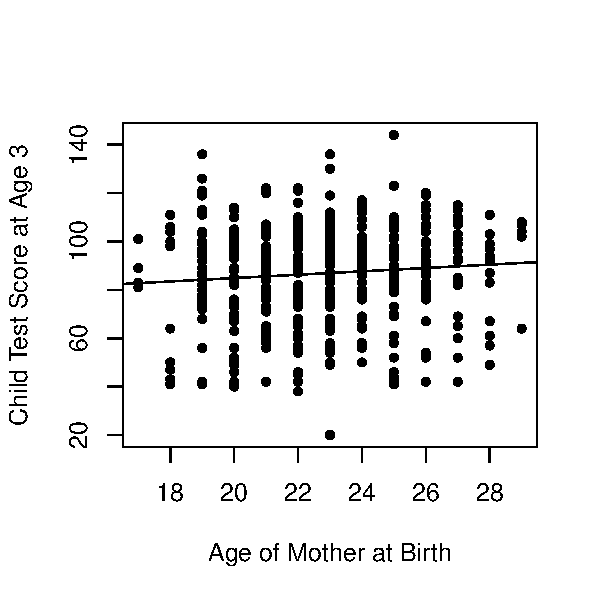
\includegraphics[width=\maxwidth]{figure/unnamed-chunk-5-1} 

}



\end{knitrout}
Our model suggests that the children of mothers who were older when they gave birth tend to score higher. In particular, comparing two children whose mothers' age at birth differed by one year, we would predict that the child of the older mother will score, on average, 0.7 points higher. The standard error associated with the estimate, however, is fairly large. An approximate 95\% CI would just barely include zero. Nevertheless, this result is suggestive that the children of older mothers do better on the test. This would seem to suggest that women should wait to have children until they are as old as possible. However, for this advice to truly be valid, it would have to be the case that being older when you give birth \emph{caused} your child to have higher test scores. This seems unlikely, since there are many possible confounders here.
    \end{solution}
		\part Augment your model from part (a) by allowing a different intercept for children whose mother completed high school. Interpret your results and compare them to those you got in part (a).
    \begin{solution}
\begin{knitrout}
\definecolor{shadecolor}{rgb}{0.969, 0.969, 0.969}\color{fgcolor}\begin{kframe}
\begin{alltt}
\hlstd{reg2} \hlkwb{<-} \hlkwd{lm}\hlstd{(kid.score} \hlopt{~} \hlstd{mom.hs} \hlopt{+} \hlstd{mom.age)}
\hlkwd{summary}\hlstd{(reg2)}
\end{alltt}
\begin{verbatim}
## 
## Call:
## lm(formula = kid.score ~ mom.hs + mom.age)
## 
## Residuals:
##     Min      1Q  Median      3Q     Max 
## -57.980 -12.545   2.057  14.709  59.325 
## 
## Coefficients:
##             Estimate Std. Error t value Pr(>|t|)    
## (Intercept)  70.4787     8.1068   8.694  < 2e-16 ***
## mom.hs       11.3112     2.3783   4.756  2.7e-06 ***
## mom.age       0.3261     0.3617   0.902    0.368    
## ---
## Signif. codes:  
## 0 '***' 0.001 '**' 0.01 '*' 0.05 '.' 0.1 ' ' 1
## 
## Residual standard error: 19.86 on 431 degrees of freedom
## Multiple R-squared:  0.05791,	Adjusted R-squared:  0.05353 
## F-statistic: 13.25 on 2 and 431 DF,  p-value: 2.614e-06
\end{verbatim}
\begin{alltt}
\hlkwd{coef}\hlstd{(reg2)}
\end{alltt}
\begin{verbatim}
## (Intercept)      mom.hs     mom.age 
##  70.4786610  11.3112315   0.3261332
\end{verbatim}
\end{kframe}
\end{knitrout}
By adding a dummy variable that equals one if a child's mother completed high school, we have controlled for one of the possible confounders from above: mother's level of education. We have done this by allowing the regression line to have a different intercept depending on mother's education. Comparing two children whose mothers are of the same age but only one whom attended high school, we predict that the child of the better educated mother will score, on average, 11.3 points higher. The standard error associated with this estimate is quite small, yielding a 95\% CI that is is nowhere near zero. We have strong evidence of a large effect from mother's education level. In contrast, once we've controlled from mother's education, the estimated effect of \texttt{mom.age} falls substantially while the associated standard error stays the same. This results in an approximate 95\% CI that includes many negative values. After controlling for mother's education, there is much less evidence to suggest that older mothers have higher-scoring children.     
\end{solution}
		\part Now allow different slopes as well as intercepts for each group (those whose mother completed high school and those whose mother did not).  Interpret your results. 
\begin{solution}
\begin{knitrout}
\definecolor{shadecolor}{rgb}{0.969, 0.969, 0.969}\color{fgcolor}\begin{kframe}
\begin{alltt}
\hlstd{reg3} \hlkwb{<-} \hlkwd{lm}\hlstd{(kid.score} \hlopt{~} \hlstd{mom.hs} \hlopt{+} \hlstd{mom.age} \hlopt{+} \hlstd{mom.hs}\hlopt{:}\hlstd{mom.age)}
\hlkwd{summary}\hlstd{(reg3)}
\end{alltt}
\begin{verbatim}
## 
## Call:
## lm(formula = kid.score ~ mom.hs + mom.age + mom.hs:mom.age)
## 
## Residuals:
##     Min      1Q  Median      3Q     Max 
## -55.535 -12.734   2.414  14.150  54.377 
## 
## Coefficients:
##                Estimate Std. Error t value Pr(>|t|)    
## (Intercept)    110.5417    16.4538   6.718 5.85e-11 ***
## mom.hs         -41.2875    18.9920  -2.174  0.03025 *  
## mom.age         -1.5220     0.7532  -2.021  0.04391 *  
## mom.hs:mom.age   2.3911     0.8567   2.791  0.00549 ** 
## ---
## Signif. codes:  
## 0 '***' 0.001 '**' 0.01 '*' 0.05 '.' 0.1 ' ' 1
## 
## Residual standard error: 19.7 on 430 degrees of freedom
## Multiple R-squared:  0.07467,	Adjusted R-squared:  0.06822 
## F-statistic: 11.57 on 3 and 430 DF,  p-value: 2.64e-07
\end{verbatim}
\begin{alltt}
\hlkwd{coef}\hlstd{(reg3)}
\end{alltt}
\begin{verbatim}
##    (Intercept)         mom.hs        mom.age mom.hs:mom.age 
##     110.541718     -41.287465      -1.522014       2.391098
\end{verbatim}
\begin{alltt}
\hlstd{intercept.no.hs} \hlkwb{<-} \hlkwd{coef}\hlstd{(reg3)[}\hlnum{1}\hlstd{]}
\hlstd{intercept.hs} \hlkwb{<-} \hlkwd{coef}\hlstd{(reg3)[}\hlnum{1}\hlstd{]} \hlopt{+} \hlkwd{coef}\hlstd{(reg3)[}\hlnum{2}\hlstd{]}
\hlstd{slope.no.hs} \hlkwb{<-} \hlkwd{coef}\hlstd{(reg3)[}\hlnum{3}\hlstd{]}
\hlstd{slope.hs} \hlkwb{<-} \hlkwd{coef}\hlstd{(reg3)[}\hlnum{3}\hlstd{]} \hlopt{+} \hlkwd{coef}\hlstd{(reg3)[}\hlnum{4}\hlstd{]}
\end{alltt}
\end{kframe}
\end{knitrout}
When we allow for different slopes as well as intercepts, by adding an \emph{interaction} between \texttt{mom.hs} and \texttt{mom.hs}, namely \texttt{mom.hs:mom.age}, we find very different results depending on mother's education. (There is strong evidence that we should allow for different slopes, since the approximate 95\% CI for the interaction does not include zero.)  For children whose mothers attended high school, there is a \emph{positive} relationship between mother's age at birth and child's test score. For children whose mothers did not attend high school, the relationship is \emph{negative}. For children whose mothers were 18 then they gave birth, there is essentially \emph{no} impact from mother's education level. As age of mother at birth increases, the impact of mother's education widens. 
\end{solution}
		\part Lastly, include mother's IQ as additional variable to the regression done in (c). Would you prefer to include mother's IQ instead of leaving it out of the regression? Compare regression results in (c) and (d). 
\begin{solution}
Mother's IQ variable is highly statistically significant. Given everything else as fixed, we predict that the child of a mother whose IQ is 1 point higher will score, on average, 1.57 points higher. After controlling for mother's IQ, mother's high school dummy and mother's age variable are not statistically significant. However, the interaction between the high school dummy and age variable still matters in the regression. Given that the mother's IQ variable has explanatory power, I would prefer to include this variable in the regression. Also, comparing adjusted R-squared and residual standard error of two regressions, regression in (d) fits the data better.
\begin{knitrout}
\definecolor{shadecolor}{rgb}{0.969, 0.969, 0.969}\color{fgcolor}\begin{kframe}
\begin{alltt}
\hlstd{reg4} \hlkwb{<-} \hlkwd{lm}\hlstd{(kid.score} \hlopt{~} \hlstd{mom.hs} \hlopt{+} \hlstd{mom.age} \hlopt{+} \hlstd{mom.hs}\hlopt{:}\hlstd{mom.age} \hlopt{+} \hlstd{mom.iq)}
\hlkwd{summary}\hlstd{(reg4)}
\end{alltt}
\begin{verbatim}
## 
## Call:
## lm(formula = kid.score ~ mom.hs + mom.age + mom.hs:mom.age + 
##     mom.iq)
## 
## Residuals:
##     Min      1Q  Median      3Q     Max 
## -53.838 -12.050   2.685  11.429  47.150 
## 
## Coefficients:
##                 Estimate Std. Error t value Pr(>|t|)    
## (Intercept)     48.47926   16.59809   2.921  0.00368 ** 
## mom.hs         -28.70540   17.48948  -1.641  0.10147    
## mom.age         -0.98470    0.69392  -1.419  0.15662    
## mom.iq           0.54865    0.06085   9.017  < 2e-16 ***
## mom.hs:mom.age   1.56800    0.79166   1.981  0.04827 *  
## ---
## Signif. codes:  
## 0 '***' 0.001 '**' 0.01 '*' 0.05 '.' 0.1 ' ' 1
## 
## Residual standard error: 18.09 on 429 degrees of freedom
## Multiple R-squared:  0.2221,	Adjusted R-squared:  0.2148 
## F-statistic: 30.62 on 4 and 429 DF,  p-value: < 2.2e-16
\end{verbatim}
\end{kframe}
\end{knitrout}
\end{solution}
	\end{parts}
	

	

\end{questions}















\end{document}
